
\normalfont

Para el método de \textit{Keele}, procederemos siguiendo el diagrama de flujo de la figura~\figref{fig:flux_diagram}. En un primer paso de cálculo, obtenemos que el primer volumen de caja obtenido para $Q_{T} = 0.303$ con la expresión:


\begin{equation}
 V_{box} = 15 \cdot Q_{T}^{2.87} \cdot V_{as}
\end{equation}


\begin{equation*}
\mathcolorbox{EQColor}{ V_{box_{Keele}} = 99.369 \si[per-mode=symbol]{\liter} }
\end{equation*}
 
 
Como volumen óptimo sin pozos o sobrepicos en la respuesta en bajas frecuencias. Al igual que con el diseño a caja cerrada, el volumen es mayor, pero aún así, aceptable para uso hogareño.\\

Proseguimos calculando los valores de frecuencia de corte y frecuencia de sintonía para el volumen obtenido, reemplazando por los valores de $Q_{T}$ requerido y $f_{s}$ del fabricante.

\begin{equation*}
f_{3} \approx 0.26 \cdot (0.303)^{-1.4} \cdot 18 \si[per-mode=symbol]{\hertz} = 25 \si[per-mode=symbol]{\hertz}
\end{equation*}

\begin{equation*}
f_{b} = 0.42 \cdot Q^{-0.9} \cdot f_{s} = 22 \si[per-mode=symbol]{\hertz}
\end{equation*}


para ser un diseño óptimo sin pozos o sobrepicos de frecuencia, consideramos que el volumen obtenido para la caja es aceptable. Ahora, según las recomendaciones del fabricante en el cuadro~\tableref{table:table_factory_recomendations}, se indica que a gabinete abierto, el volumen recomendado es de $V_{box} = 129 \si[per-mode=symbol]{\liter} $ con $f_{b} = 20 \si[per-mode=symbol]{\hertz}$ y $f_{3} = 21 \si[per-mode=symbol]{\hertz}$. A un volumen mas grande, tenemos una menor frecuencia de corte. Verificando con el método de Keele, obtenemos que:


\begin{equation}
f_{3_{Keele}} = \sqrt{\frac{V_{as}}{V_{box}}} \cdot f_{s}
\end{equation}


\begin{equation*}
\mathcolorbox{EQColor}{ f_{3_{Keele}} = 22.63 \si[per-mode=symbol]{\hertz} }
\end{equation*}

\begin{equation}
f_{b_{Keele}} = \left( \frac{V_{as}}{V_{box}} \right)^{0.32} \cdot f_{s}
\end{equation}


\begin{equation*}
\mathcolorbox{EQColor}{ f_{b_{Keele}} = 20.84 \si[per-mode=symbol]{\hertz} }
\end{equation*} \\

que no difiere demasiado, pero según \textit{Keele}, tenemos un pozo en la respuesta en frecuencia:

\begin{equation}
Hump_{\si[per-mode=symbol]{\decibel}} = 20 \cdot log \left( 2.6 \cdot Q_{T} \cdot \left( \frac{V_{as}}{V_{box}} \right)^{0.35} \right)
\end{equation}

\begin{equation*}
\boxed{ Hump_{\si[per-mode=symbol]{\decibel}} = -0.68 \si[per-mode=symbol]{\decibel} }
\end{equation*}

Que dado su valor, se puede despreciar. \\



%% \noindent
%% \begin{center}
 
%%\begin{spacing}{1}  
\begin{table}[H]  %%\centering

    \setlength\arrayrulewidth{1.5pt}
    \arrayrulecolor{white}
    \def\clinecolor{\hhline{|>{\arrayrulecolor{white}}-%
    >{\arrayrulecolor{white}}|-|-|-|}}
\resizebox{0.98 \textwidth}{!}{% 
       
\begin{tabularx}{1 \textwidth}%
    {|
    >{\columncolor{white} \centering\arraybackslash}m{0.20\textwidth}
     |
    >{\columncolor{white} \centering\arraybackslash}m{0.35\textwidth}
     |
    >{\columncolor{white} \centering\arraybackslash}m{0.45\textwidth}
     |
    }
    \rowcolor{EQColor} \thead{Parámetro}  & \thead{Recomendado} & \thead{Diseñado} \\    
    \hhline{|-|-|-|}
    \rowcolor{gray!20} \cellcolor{gray!40} $V_{box}$ &  $129 \si[per-mode=symbol]{\liter}$ & $99.369 \si[per-mode=symbol]{\liter}$ \\  
    \hhline{|-|-|-|}  
    \rowcolor{gray!20} \cellcolor{gray!40} $f_{3}$ & $21 \si[per-mode=symbol]{\hertz}$ & $22.63 \si[per-mode=symbol]{\hertz}$ \\
    \hhline{|-|-|-|}  
    \rowcolor{gray!20} \cellcolor{gray!40} $f_{b}$ & $22 \si[per-mode=symbol]{\hertz}$ & $20.84 \si[per-mode=symbol]{\hertz}$ \\  
    \end{tabularx}}
	\caption{\footnotesize{Comparación de los valores diseñados (\textit{keele}) con los recomendados por el fabricante.}}
	\label{table:table_comparison_keele_recomendations}
\end{table}
%%\end{spacing}

Con los valores diseñados, recordando que tiene que contener el parlante de $32 \si[per-mode=symbol]{\centi\meter}$ de diámetro y $15 \si[per-mode=symbol]{\centi\meter}$ de largo, podemos calcular las dimensiones de la caja.

Si hacemos el largo de $33 \si[per-mode=symbol]{\centi\meter}$ para acomodar el diámetro del parlante, y redondeando el volumen obtenido a $100000 \si[per-mode=symbol]{\cubic\centi\meter}$, haciendo la base cuadrada obtenemos:


\begin{equation*}
Alto = Ancho = \sqrt{\frac{V_{box}}{Largo}} = \sqrt{\frac{100000 \si[per-mode=symbol]{\cubic\centi\meter}}{33 \si[per-mode=symbol]{\centi\meter}}} = 55.048 \si[per-mode=symbol]{\centi\meter} \approx 55 \si[per-mode=symbol]{\centi\meter}
\end{equation*}

Finalemente obtenemos:


\begin{mymathbox}[ams align*, title=Dimensiones de la caja (método de \textit{Keele}), colframe=EQColor!30!EQColor]
Alto = 55 \si[per-mode=symbol]{\cubic\centi\meter} \\
Ancho = 55\si[per-mode=symbol]{\cubic\centi\meter} \\
Largo = 33 \si[per-mode=symbol]{\cubic\centi\meter}
\end{mymathbox}


\vfill


\clearpage

\begin{figure}[H]
	\centering
	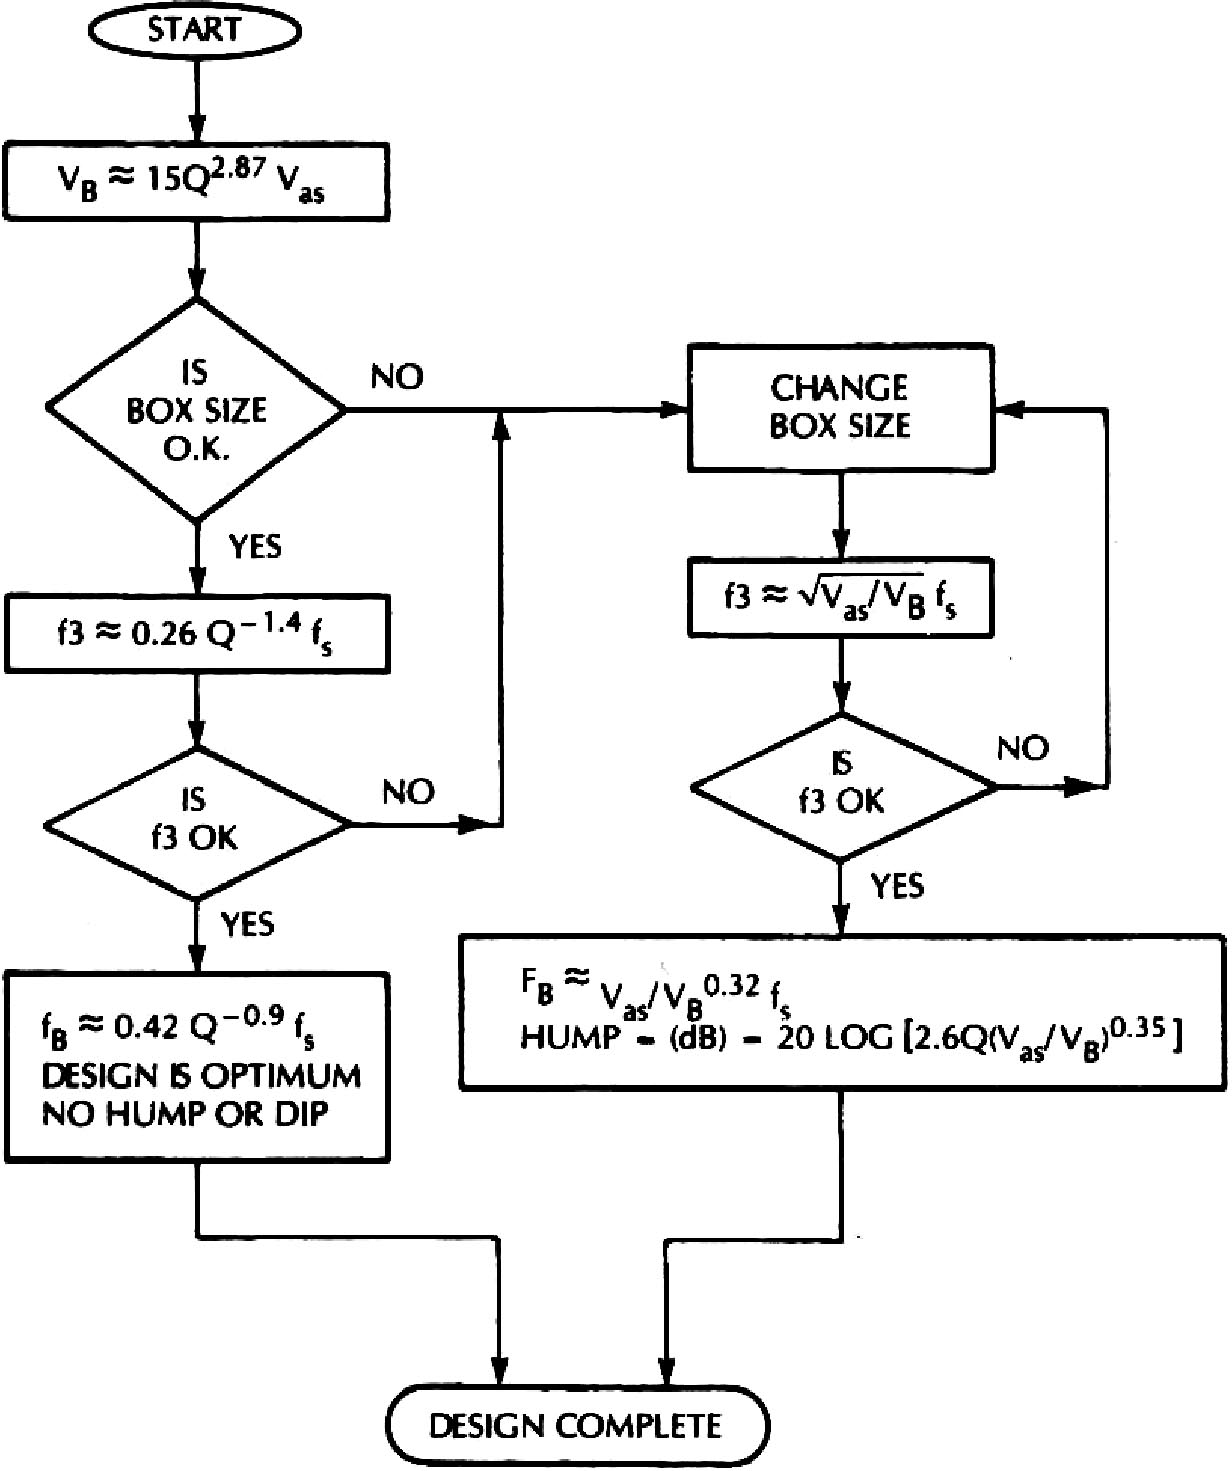
\includegraphics[width=1\textwidth]{./img/diag/keele.png}
	\caption{Digrama de flujo para diseño de \textit{Keele}.}
	\label{fig:flux_diagram}
\end{figure}